% Transferner -- CSCE 883 Project Proposal (2 pages max)
% Compile on Overleaf (pdfLaTeX) or locally: pdflatex -> bibtex -> pdflatex x2
\documentclass[conference,10pt]{IEEEtran}
\usepackage[T1]{fontenc}
\usepackage{graphicx}
\usepackage{booktabs}
\usepackage{xcolor}
\usepackage{amsmath,amssymb}
\usepackage{tikz}
\usetikzlibrary{positioning,arrows.meta}
\usepackage[hidelinks]{hyperref}
\usepackage{url}
\newcommand{\TBD}[1]{\textcolor{red}{[#1]}}

\begin{document}
\bstctlcite{IEEEexample:BSTcontrol}

\title{Transferner: Risk-Aware, On-Device Identification of Edible Plants and Their Toxic Look-Alikes in the Southeastern United States}

\author{%
\IEEEauthorblockN{Jacob Bagley}
\IEEEauthorblockA{University of South Carolina\\ jccbagley@protonmail.com}
\and
\IEEEauthorblockN{EmmaLee Peyton}
\IEEEauthorblockA{University of South Carolina\\ emmaleejp@gmail.com}
}
\maketitle

% =====================================================================
\section{Problem Statement and Significance}
People with limited botanical knowledge may rely on phone apps to decide whether a
wild plant is safe to forage. In a clinical-toxicology evaluation of four popular
apps, species-level accuracy was 58\%, and five of eleven potentially toxic species
were identified as an edible species by at least one app~\cite{long2023midwest}.
Standard classifiers treat all errors equally, yet calling poison hemlock wild carrot is far
worse than the reverse. We cover $\sim$1{,}000 regional species while explicitly targeting \emph{toxic
look-alikes} and the asymmetric cost of errors.

We will build \textbf{Transferner}, an Android app for South Carolina and neighboring
states (North Carolina, Georgia, and Tennessee). A lightweight MobileNetV4 model, designed to be mostly Pareto-optimal across mobile CPUs,
DSPs, GPUs, and the Pixel EdgeTPU~\cite{qin2024mobilenetv4}, runs live on the camera feed. When the user captures a still image, BioCLIP~2.5
Huge, the ViT-H/14 successor to BioCLIP~2~\cite{gu2025bioclip2}, identifies the plant. The app returns a species
prediction, contact and ingestion toxicity flags, and an explicit ``not sure---possible toxic look-alike''
response instead of a confident wrong answer. Our research question:
\emph{Which adaptation and compression techniques (LoRA, partial INT8 quantization,
etc.) preserve or improve toxic/edible discrimination under a phone's latency and
memory budget?}

% =====================================================================
\section{Data}
\textbf{Sources.} (i) Pl@ntNet observations from GBIF~\cite{gbif_plantnet_obs}
(records CC~BY~4.0; each photo carries its own license), filtered by GADM state;
the four states hold $\sim$13.9K photographed observations (Oct.~2026); and
(ii) TreeOfLife-200M~\cite{gu2025bioclip2}, which combines GBIF, EOL, BIOSCAN-5M, and
FathomNet into 214M images of 952,257 taxa.
It ships metadata and URLs, so we download only our target species.

\textbf{Scope.} About 1{,}000 regional species. Most have no meaningful visual overlap
with a toxic species and are trained as ordinary classes; a subset forms
toxic/edible look-alike groups that receive targeted data and evaluation, e.g.,
poison hemlock (\emph{Conium maculatum}) vs.\ wild carrot (\emph{Daucus carota});
water hemlock (\emph{Cicuta maculata}) vs.\ wild carrot and elderberry
(\emph{Sambucus canadensis}); Canada moonseed (\emph{Menispermum canadense}) and
pokeweed (\emph{Phytolacca americana}) fruit vs.\ wild grapes incl.\ muscadine
(\emph{Vitis} spp.); and, for contact toxicity, poison ivy (\emph{Toxicodendron
radicans}) vs.\ blackberry/raspberry (\emph{Rubus} spp.). Each pair is documented
as a confusion by extension or poison-center sources.
Toxicity labels (humans only) are \emph{independent} binary contact and ingestion
flags derived from the NC State Extension Plant Toolbox: contact from its ``Causes
Contact Dermatitis'' field, ingestion from its poison severity and symptoms.

\textbf{Size and splits.} About 200 images per toxic and look-alike species, drawn from
both TreeOfLife-200M and Pl@ntNet;
70/15/15 train/val/test split by \emph{observation}, so that photos of the same
plant never appear in two splits; test observations come only from the
leakage-free pool below.

\textbf{Leakage control.} BioCLIP~2/2.5 were pretrained on TreeOfLife-200M, so test
images drawn from it would inflate scores. Our test set will use Pl@ntNet/GBIF records
\emph{not} in the TreeOfLife-200M catalog (matched by source ID, plus perceptual-hash
de-duplication) or records newer than its snapshot.

\textbf{Known issues.} Long-tailed class counts, label
noise in citizen-science data, and appearance that changes with growth stage
(seedling, flower, fruit).

% --- Example-image figure (required by the course: "dataset with examples") ---
\begin{figure}[t]
\centering
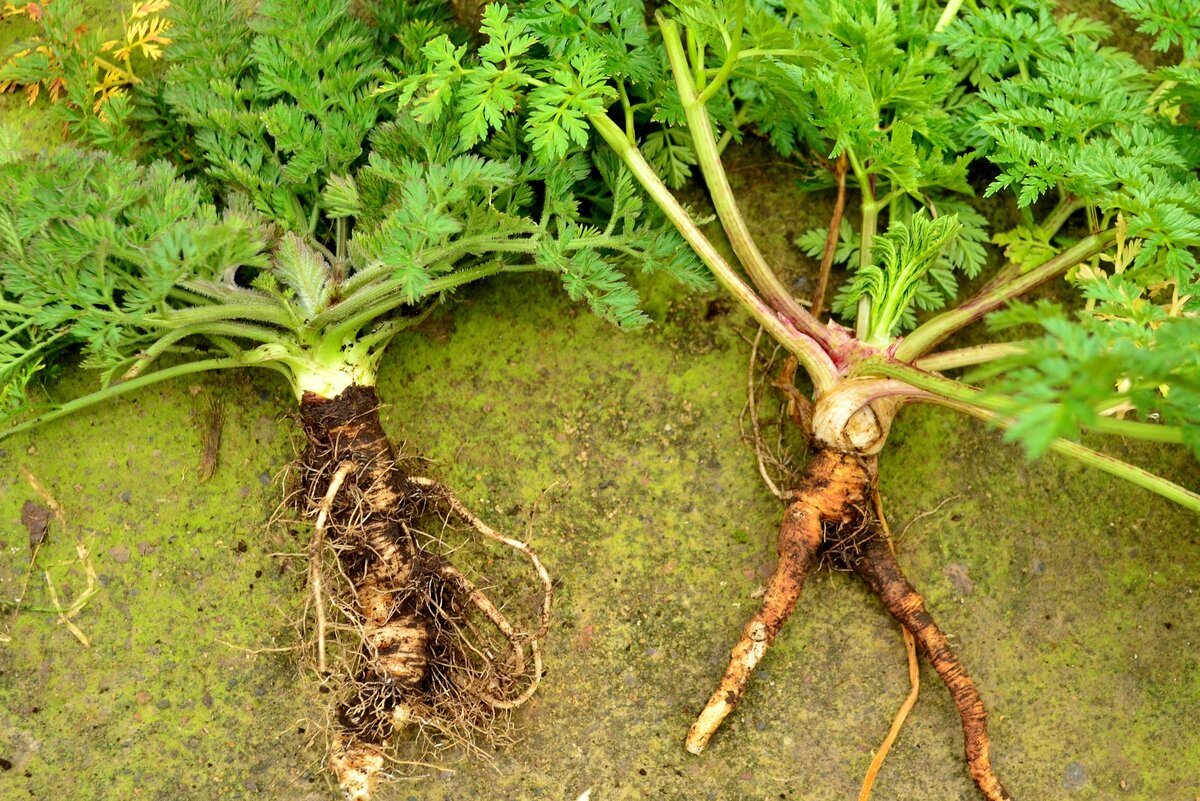
\includegraphics[width=0.82\columnwidth]{figs/carrot_vs_hemlock_holly.jpg}
\caption{Young plants of a look-alike pair: wild carrot (\emph{D.~carota}, left;
root edible when young, hairy stem) vs.\ poison hemlock (\emph{C.~maculatum}, right; toxic,
hairless stem with purple blotching). Photo \copyright~2015 H.~Holly, used with
credit~\cite{holly2026carrot}.}
\label{fig:pair}
\end{figure}

% =====================================================================
\section{Proposed Method}
\textbf{Two-stage pipeline.}
\emph{Stage~1 (live):} MobileNetV4~\cite{qin2024mobilenetv4} is fine-tuned from ImageNet weights (timm) on our
$\sim$1{,}000-way regional label set. Stage~1 runs per frame to give a live top-$k$ guess
and to warn early when a look-alike group is in view.
\emph{Stage~2 (still image):} BioCLIP~2.5 Huge (CLIP-style ViT-H/14, loaded with OpenCLIP)
classifies the still image. Text embeddings for our label set are computed offline, so
only the roughly 632M-parameter image encoder runs at inference.
At 632M parameters its weights alone occupy $\sim$1.26\,GB in FP16 versus
$\sim$0.63\,GB in INT8, which is why quantization is required, not optional, for
on-device use. Fig.~\ref{fig:pipe} summarizes the pipeline.
\textbf{All app inference runs on the edge device}; servers are used only for training and
lab testing.

\begin{figure}[t]
\centering
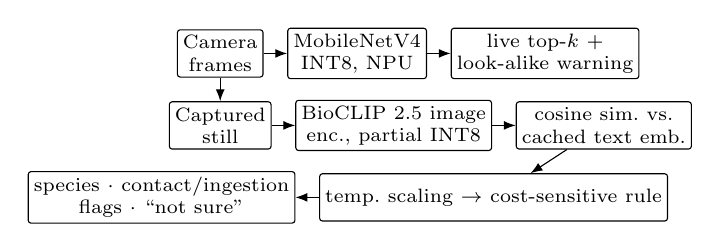
\begin{tikzpicture}[font=\scriptsize, node distance=3mm and 3mm,
  box/.style={draw, rounded corners=1pt, align=center, inner sep=2pt, minimum height=6mm},
  arr/.style={-{Latex[length=1.5mm]}}]
\node[box] (cam) {Camera\\frames};
\node[box, right=of cam] (mnv4) {MobileNetV4\\INT8, NPU};
\node[box, right=of mnv4] (live) {live top-$k$ +\\look-alike warning};
\node[box, below=of cam] (still) {Captured\\still};
\node[box, right=of still] (bc) {BioCLIP~2.5 image\\enc., partial INT8};
\node[box, right=of bc] (sim) {cosine sim.\ vs.\\cached text emb.};
\node[box, below=of sim, xshift=-14mm] (dec) {temp.\ scaling $\rightarrow$ cost-sensitive rule};
\node[box, left=of dec] (out) {species $\cdot$ contact/ingestion\\flags $\cdot$ ``not sure''};
\draw[arr] (cam) -- (mnv4); \draw[arr] (mnv4) -- (live);
\draw[arr] (cam) -- (still);
\draw[arr] (still) -- (bc); \draw[arr] (bc) -- (sim);
\draw[arr] (sim) -- (dec); \draw[arr] (dec) -- (out);
\end{tikzpicture}
\caption{On-device pipeline. All inference runs on the phone; text embeddings for
the $\sim$1{,}000 labels are computed once offline.}
\label{fig:pipe}
\end{figure}

\textbf{Techniques we will compare.}
\begin{itemize}
\item \textbf{Zero-shot baselines:} BioCLIP, BioCLIP~2, and BioCLIP~2.5.
\item \textbf{LoRA}~\cite{hu2022lora} on the BioCLIP~2.5 image encoder (via
Hugging Face PEFT), compared against a linear probe on frozen features;
MobileNetV4 is fully fine-tuned.
\item \textbf{Look-alike-focused training:} class-balanced loss
for the long tail.
\item \textbf{Partial INT8 quantization}~\cite{nagel2021whitepaper}:
post-training and quantization-aware INT8. Layers whose quantization error most raises
toxic-class confusion stay at FP16.
\item \textbf{Risk-aware decision:} temperature scaling~\cite{guo2017calibration}
gives calibrated $p_i=\mathrm{softmax}(z/T)_i$. With cost $C_{ij}$ for predicting $j$
when the truth is $i$ (large when $i$ is toxic and $j$ is not), the app outputs
$\hat{y}=\arg\min_j \sum_i C_{ij}\,p_i$, or ``not sure'' when that minimum expected cost
exceeds an abstention cost $c_a$. $C$ and $c_a$ are tuned on validation data.
\end{itemize}

\textbf{Implementation.} Training uses PyTorch on an AMD
Radeon RX~7900~XTX (24\,GB, gfx1100), which ROCm officially supports on
Linux. Models are exported with LiteRT
Torch to LiteRT and run on a Google Pixel phone, using the NPU and CPU in
tandem. LiteRT's Google Tensor NPU path is in beta and
supports ahead-of-time compilation only, so CPU/GPU execution is our
fallback.
Code: \url{https://github.com/CyberneticMedic/Transferner}.
\textbf{Roles:} J.~Bagley---data, training, quantization, on-device benchmarking;
E.~Peyton---app front end/UX, safety-message design, report.

% =====================================================================
\section{Evaluation and Expected Results}
\textbf{Headline metric---dangerous miss rate (DMR):} with $\mathcal{T}$
the toxic classes and $\mathcal{D}_\mathcal{T}$ the test images whose true class is toxic,
$\mathrm{DMR}=|\{x\in\mathcal{D}_\mathcal{T}:\hat{y}(x)\notin\mathcal{T}\cup\{\text{not sure}\}\}|\,/\,|\mathcal{D}_\mathcal{T}|$,
i.e., toxic plants the app confidently calls non-toxic. It is computed separately with
$\mathcal{T}$ as the contact-toxic and the ingestion-toxic set. We report it overall and per look-alike pair.
\textbf{Other metrics:} top-1/top-5 accuracy, macro-F1, expected calibration error
(ECE, overall and on toxic classes), coverage at fixed DMR, on-device latency
(NPU vs.\ CPU), model size, and peak memory. Lab tests run on held-out data; deployment tests are \emph{field-based}, photographing
plants in situ in the target region. We give 95\% bootstrap confidence
intervals and use McNemar's test to compare paired model variants.
\textbf{Expected figures:} look-alike confusion matrices; reliability diagrams before
and after calibration; risk--coverage curves; and an accuracy/DMR vs.\ latency
Pareto plot across FP32, partial-INT8, and full-INT8 models.
\textbf{Hypotheses:} (H1) LoRA-adapted BioCLIP~2.5 lowers DMR versus zero-shot.
(H2) Full INT8 hurts look-alike pairs more than overall accuracy; partial INT8 recovers
most of the loss. (H3) Calibration plus abstention cuts DMR at a modest coverage cost.

% =====================================================================
\textbf{Risks and fallbacks.} (i) Google Tensor NPU support is beta: fall back to
GPU/CPU delegates and report per-unit latency. (ii) Regional Pl@ntNet data is thin
($\sim$14 observations/species on average): supplement from TreeOfLife-200M and report
per-source accuracy. (iii) BioCLIP~2.5 too slow on-device even at INT8: distill it
into MobileNetV4, or use BioCLIP~2 (ViT-L/14) as the still-image model.

\section{Timeline (Proposed)}
{\centering\footnotesize
\begin{tabular}{@{}lp{0.72\columnwidth}@{}}
\toprule
\textbf{Dates} & \textbf{Milestone} \\ \midrule
Oct 19--25 & Project coordination and planning; repository setup; species list and toxicity labels; data scripts \\
Oct 26--Nov 1 & Dataset built and split; zero-shot BioCLIP and MNv4 baselines; app camera + LiteRT skeleton \\
Nov 2--15 & LoRA on BioCLIP~2.5; class-balanced MNv4; calibration, cost rule, abstention; app result/warning UI \\
Nov 16--22 & INT8 (PTQ/QAT, partial); LiteRT export; Pixel NPU/CPU benchmarks \\
Nov 23--29 & Full evaluation, failure analysis (Thanksgiving buffer) \\
Nov 30--Dec 10 & Report, demo video, slides; rehearse; present Dec 10; submit zip \\ \bottomrule
\end{tabular}\par}

\footnotesize
\bibliographystyle{IEEEtran}
\bibliography{references}
\end{document}
